\chapter{User Interface}
Developer: Yann

\noindent Validator: All


%DEVELOPER WRITES THIS PART --->

\section{Requirements}

We wanted to have a quick and efficient user interface to be able to provide the user with what is in the beast, both play with products independantly of aggregate them in a portfolio. If also does the import for data files (see the help menu on file formatting), and enables the user to check the tests we ran in C++ to view the robustness of our objects.

\section{Main }

Lauching the executable \textit{terreneuve-exe} leads the user to the main menu:

\begin{figure}[htbp]
\begin{center}
        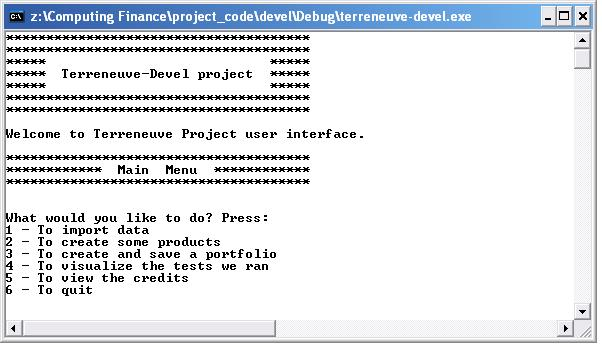
\includegraphics[width=11cm]{mainmenu.jpg}
        \caption{Main menu interface}
\end{center}
\end{figure}

From there he can 
\begin{enumerate}
	\item Import some data -- required for the options 2 and 3, the user can import our default data if he wants.
	\item Create some products -- all except the variance swap.
	\item Create/Retrieve a portfolio of all the products -- not available, but uses the option 2: all the existing menus to create a product in (2) return the object they created, so the adding of this functionnality to the user menu would be quick.
	\item Have a look at the C++ hard coded tests the coders ran to check their objects.
	\item Credits -- what is a GNU module without this !
	\item Quit -- which is too soon ... 
\end{enumerate}

\section{Import }

The import menu is straight forward -- here the user has chosen the default data. Else he has a menu to input the directory in which he has the data. An help menu on the file formats we used is available. Note that if the user wants flat rates, credit spreads and volatility, he should import the default data, as in all the menus the program asks him once more if he wants to use the data or enter flat curves.

\begin{figure}[htbp]
\begin{center}
        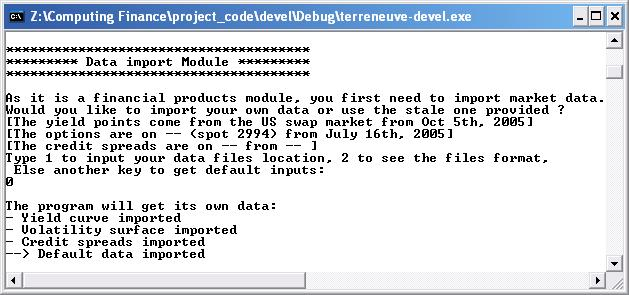
\includegraphics[width=12cm]{importDefault.jpg}
        \caption{Import data interface}
\end{center}
\end{figure}

\section{Products}

Once the import has been done, the user can create products and look at how they behave. If he wants to use flat curves, again he is being asked.

\begin{figure}[htbp]
\begin{center}
        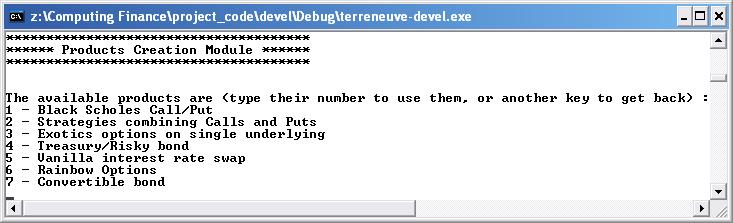
\includegraphics[width=12cm]{products.jpg}
        \caption{Products interface}
\end{center}
\end{figure}

The rest is very user friendly to create the products and view their sensitivities.


\section{Portfolio}

This has not been done in the menu, but as we said, it can be coded really quickly by using each product console input module and its functions:
\begin{enumerate}
	\item BlackScholes* inputBSOption(marketData data);
	\item OptionStrategy inputOptionStrategy(marketData data);
	\item Exotics* inputExoticOptionOnSingleAsset(marketData \&data);
	\item bond* inputBond(marketData \&data);
	\item VanillaSwap* inputVanillaSwap(marketData data);
	\item RainbowOption* inputRainbowOption(marketData data);
	\item convertiblebond* inputConvertibleBond(marketData \&data);
\end{enumerate}



\section{Credits}

Working together for 2 months leaves scars ... actually, it leaves anecdotes, so we tried to have the user share some of them.

Just select this option and you will see.




\section{Quit}

Come on, not yet, it is just the beginning of the report.